% Chapter 4: Thermodynamic Maps
% Source: papers/thermodynamic-maps-pnas/Research_report.tex

% Use letters for affiliations, numbers to show equal authorship (if applicable) and to indicate the corresponding author

% Please give the surname of the lead author for the running footer

% Please add a significance statement to explain the relevance of your work

% Please include corresponding author, author contribution and author declaration information

To whom correspondence should be addressed. E-mail: ptiwary\@umd.edu}

% At least three keywords are required at submission. Please provide three to five keywords, separated by the pipe symbol.

}

\ifthenelse{\boolean{shortarticle}}{\ifthenelse{\boolean{singlecolumn}}{\abscontentformatted}{\abscontent}}{}

% Use \firstpage to indicate which paragraph and line will start the second page and subsequent formatting. In this example, there are a total of 11 paragraphs on the first page, counting the first level heading as a paragraph. The value {12} represents the number of the paragraph starting the second page. If a paragraph runs over onto the second page, include a bracket with the paragraph line number starting the second page, followed by the paragraph number in curly brackets, e.g. "".

% If your first paragraph (i.e. with the \dropcap) contains a list environment (quote, quotation, theorem, definition, enumerate, itemize...), the line after the list may have some extra indentation. If this is the case, add \parshape=0 to the end of the list environment.
\label{ch4:sec:intro}

% \subsection{Free Energy Landscapes and Phase Transitions}

hase transitions are widely observed in biological, material, and social sciences. Across these disciplines, phase transitions can be defined as the emergence of higher-level, large-scale organization from the coordinated, short-range interactions between many individual constituents. Classical examples include the ferromagnetic to paramagnetic transition, boiling of water, and conformational transitions in biomolecules like proteins and nucleic acids.

Statistical mechanics, and especially the framework of energy landscapes, provides a simple and unifying way of studying phase transitions in these diverse systems \cite{wales-energy-landscapes}. In this work we are specifically interested in phase transitions in systems that stay in equilibrium throughout. For these, the Boltzmann distribution relates the probability of finding a system in a particular microscopic configuration $\mathbf{x}$ to its energy $U(\mathbf{x})$ and the system's inverse temperature $\beta$ as
\begin{equation}
\label{ch4:eq:boltzmann}
\mu(\mathbf{x},\beta) = \frac{e^{ -\beta U(\mathbf{x})}}{Z(\beta)} \quad \text{with}
\end{equation}

\begin{equation}
\label{ch4:eq:partition-func}
Z(\beta) = \int e^{-\beta U(\mathbf{x})} d\mathbf{x}. 
\end{equation}

$Z(\beta)$ is a normalization constant known as the partition function, whose behavior is often associated with phase transitions. Exploration of the energy landscape is guided by competition between energy and entropy, which is encapsulated by a temperature-dependent free energy $F(\beta)$ which may be computed from the partition function as
\begin{equation}
    \label{ch4:eq:free-energy}
    F(\beta) = -\beta^{-1} \ln Z(\beta).
\end{equation}

At a glance, Eqs. \ref{ch4:eq:boltzmann}-\ref{ch4:eq:free-energy} suggest that the relationship between temperature, energy, microscopic probability, and macroscopic free energy is simple and tractable. It appears as if with these equations, one has the machinery to directly calculate the free energy across temperatures. By doing so for different macroscopic phases one could then obtain various thermodynamic attributes of phase transitions, including transition temperatures and phase diagrams. By calculating appropriate fluctuations, one could directly obtain response functions such as heat capacities.

In reality, however, the situation is quite complex. Studying phase transitions and their characteristics computationally is made difficult by Eq. \ref{ch4:eq:partition-func}, which requires integrating over a (usually) intractably large number of dimensions. Numerous
elegant theoretical and computational schemes have been proposed over the decades to solve this problem. For example, this includes methods like free energy perturbation, Markov chain Monte Carlo (MC) methods,  the replica trick and others \cite{zwanzig-fep,monte-carlo-review,wham,bar,mbar,parisi-replica-trick}.

In this study, we propose a generative Artificial Intelligence (AI) based approach that characterizes phase transitions by effectively learning the temperature dependence of the partition function, and therefore the free energy. Our method, which we call ``thermodynamic maps'' (TM) incorporates score-based generative modeling into the framework of free energy perturbation within statistical mechanics \cite{nonequilibrium-learning,ddpm,score-based-generative,ddpm-remd}. The central idea underlying thermodynamic maps is to map the temperature dependence of configurational ensembles of a complex system to and from the temperature dependence of a simple, idealized system. We show how such a bidirectional mapping can be obtained. This allows for efficient generation of physically realistic samples of the complex system with the correct Boltzmann weights. Within the framework of free energy perturbation, the mapping also allows for temperature-dependent free energy estimates. 

We demonstrate the broad applicability of thermodynamic maps for three complex systems where we compare against benchmarks from theory, extensive computational studies, and experiments. The first system we consider is the Ising model on a two-dimensional square lattice. With observations made at two temperatures, one deep in the paramagnetic regime and the other deep in the ferromagnetic regime, we are able to correctly infer critical behavior. We then study two different Ribonucleic Acid (RNA) systems: the GCAA tetraloop and HIV-TAR RNA \cite{gcaa-nmr,hiv-nmr}. For both of these, we infer the temperature-dependence of the equilibrium distribution across temperatures using thermodynamic maps trained on data generated by short molecular dynamics (MD) simulations. For both RNA systems, we predict the temperature dependence of conformational ensemble and compute melting temperatures, finding agreement with computational studies and experiment.

Given this demonstration of applicability, we believe that thermodynamic maps will be found useful for the characterization of complex phase transitions in diverse systems, especially those with multiple phases. For example, local minima within the energy landscape of biomolecular systems are often biologically and functionally relevant \cite{excited-states}, and while they have been historically challenging to characterize computationally, we are able to study them with thermodynamic maps. The computational efficiency of the learning algorithm and scalability due to not requiring samples from the global equilibrium distribution make thermodynamic maps especially suitable for studying large-scale systems exhibiting complex behavior across long timescales.

\section{Method}

\subsection{Targeted Free Energy Perturbation}
\label{ch4:sec:TFEP}

% \subsubsection{Targeted Free Energy Perturbation}

%To better understand phase transitions one must first understand the behavior of the free energy, which amounts to estimating the partition function. 

To motivate thermodynamic maps, we start with relevant background work in the longstanding problem of free energy estimation. Since pioneering work by Zwanzig and Feynman in the 1950s, many frameworks have been developed to do this efficiently \cite{zwanzig-fep,feynman,TI,mbar,bar}. The guiding principle behind all such methods is that one is usually interested in differences of free energies, rather than their absolute values. Such differences can be estimated from ratios of partition functions.
One relatively recent framework is that of Targeted Free Energy Perturbation (TFEP), which is especially relevant for machine learning approaches to free energy estimation \cite{TFEP}. 

Estimates of free energy differences between states converge according to the overlap between the states. Avoiding a technical definition, the overlap between states $A$ and $B$ measures how likely it is to generate a sample from $B$ by sampling from $A$. The central idea behind TFEP is to increase the overlap between states with an invertible mapping of the configuration space onto itself:
\begin{equation}
    \label{ch4:eq:TFEP-mapping}
    \mathcal{M}:\mathbf{x}\rightarrow\mathbf{x}'.
\end{equation}
A well-chosen $\mathcal{M}$ might map $\mathbf{x} \in A$ so that $A'$ is a subset of $B$. Under such a mapping, sampling from $A$ and transforming the sample using Eq. \ref{ch4:eq:TFEP-mapping} always generates a sample from $B$; it is therefore more efficient to estimate free energies under $\mathcal{M}$ and reweight back to the original configuration space. Reweighting is possible if $\mathcal{M}$ has a well-defined Jacobian $J_\mathcal{M}$ by using the following property: if $p(\mathbf{x})$ is the probability density of $\mathbf{x} \in A$ and $q(\mathbf{x}')$ of $\mathbf{x}' \in A'$, then the densities are related through the identity

\begin{equation}
    \label{ch4:eq:normalization}
    p(\mathbf{x}) = \frac{q(\mathbf{x}')}{| \det J_{\mathcal{M}}(\mathbf{x}')|}.
\end{equation}
Using Eq. \ref{ch4:eq:normalization} free energy differences computed under $\mathcal{M}$ can be reweighted to free energy differences in the original configuration space.

Clearly using Eqs. \ref{ch4:eq:TFEP-mapping} and \ref{ch4:eq:normalization} depends on specifying a map that increases the overlap between states and has a tractable Jacobian. Finding a suitable mapping is difficult due to the often complex, high-dimensional nature of the configurations; as a result, the most successful approaches to TFEP represent $\mathcal{M}$ with a neural network \cite{tfep-2020,LFEP}. Likelihood-based models have been especially appealing since they meet both conditions \cite{NFReview,RealNVP,NeuralODE}, but have drawbacks of reduced expressivity and robustness \cite{bbvi}. Recent lines of work have improved both aspects -- for example, by pursuing more expressive black-box operations or incorporating stochasticity \cite{smooth-NF,neural-spline,AIS-NF,StochasticNF}. In the following sections, we bypass these issues of finding a suitable mapping by exploring non-equilibrium diffusion processes as general-purpose maps.

\subsection{Leveraging Non-Equilibrium Thermodynamics}
\label{ch4:sec:FPE}

\begin{figure}
    \centering
    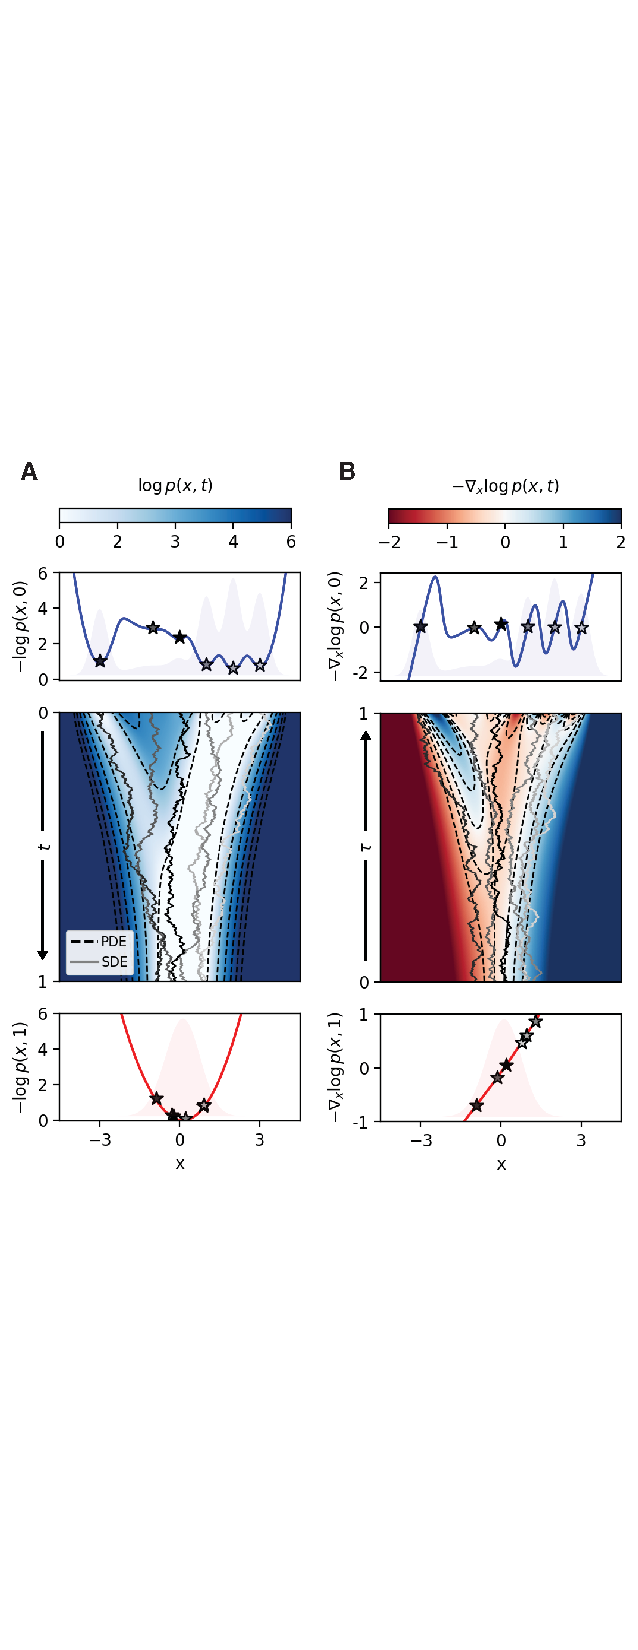
\includegraphics[
    width=0.45\textwidth
    ]{figures/ch4_OU-process.pdf}
    \caption{ {\bf Transporting a probability distribution with a diffusion process.} {\bf A} The top panel shows the negative log-likelihood for a mixture of Gaussians. The center panels show the dynamics of a diffusion process defined as a PDE (contours) and an SDE (solid lines). Over a time interval from 0 to 1 the diffusion process relaxes to a Gaussian distribution. {\bf B} The same dynamics are depicted in terms of the score. In both panels, the dynamics of the diffusion process can be viewed forward or backward in time (denoted by $t$ and $\tau$ respectively).}
    \label{ch4:fig:OU}%
\end{figure}

We begin by recounting the main results of a line of work that explores using properties of stochastic processes for general inference \cite{hyvarinen-score,nonequilibrium-learning,song-2019,score-based-generative,FPE-score-maoutsa,FPE-probability-flow}. Suppose that the diffusion process is modeled as a Fokker-Planck equation cast in the form of a Liouville equation

\begin{equation}
    \frac{\partial}{\partial t}p(\mathbf{x},t) = -\lambda(t) \nabla \cdot  \left[b(\mathbf{x},t) p(\mathbf{x},t) \right] \; \mathrm{with}
    \label{ch4:eq:FPE-PDE} 
\end{equation}
\begin{equation}
    b(\mathbf{x},t) = \mathbf{x} - \nabla \log p(\mathbf{x},t),
    \label{ch4:eq:vector-field} 
\end{equation}

where gradients are assumed to be with respect to spatial coordinates $\mathbf{x}$ \cite{FPE-probability-flow,fokker-planck}. Eq. \ref{ch4:eq:FPE-PDE} is a partial differential equation (PDE) describing the evolution of a probability distribution $p(\mathbf{x},t)$ towards a Gaussian distribution under the influence of the vector field $b(\mathbf{x},t)$ (Eq. \ref{ch4:eq:vector-field}). Time is dilated by the noise schedule $\lambda(t)$ -- a monotonically increasing scalar-valued function that ensures the process converges sufficiently close to a Gaussian distribution at $t=1$. Equivalently, the process can be expressed in terms of the evolution of a particle using a stochastic differential equation (SDE) of the form

\begin{equation}
    \mathrm{d}\mathbf{x} = -\lambda(t)\mathbf{x}\mathrm{d}t + \sqrt{2\lambda(t)}\mathrm{d}\mathbf{B}_t,
    \label{ch4:eq:FPE-SDE}
\end{equation}
where $\mathbf{B}_t$ is a standard Brownian motion and $\mathbf{x}$ is implicitly a function of $t$. 

In Figure \ref{ch4:fig:OU} we solve Eqs. \ref{ch4:eq:FPE-PDE} and \ref{ch4:eq:FPE-SDE} numerically in one spatial dimension. Figure \ref{ch4:fig:OU}A shows the solution of Eq. \ref{ch4:eq:FPE-PDE} when $p(x,0)$ is a mixture of Gaussians. In this case, it is possible the evaluate the PDE exactly since $\log p(x,t)$ is known for all $t$. The dynamics of Eq. \ref{ch4:eq:FPE-PDE} are presented in the center panel, where an initial distribution is transported to a single Gaussian; during the process the barriers that originally separated the states are destroyed. Similarly, the trajectories generated by the SDE begin at points on $\log p(x,t)$ (marked as stars) and end in a Gaussian distribution at $t=1$. The diffusion process demonstrably increases overlap by mapping all states onto a single reference state, and does so for arbitrary initial conditions. However, if the diffusion process is to be a valid TFEP map it must meet the invertibility requirement in Section \ref{ch4:sec:TFEP}

Indeed, Eq. \ref{ch4:eq:FPE-PDE} is invertible under the time-reversal $\tau \equiv 1 - t$. Remarkably, it can be shown that the time-reverse of Eq. \ref{ch4:eq:FPE-SDE} also exists \cite{Anderson1982} and is an SDE  of the form

\begin{equation}
    \mathrm{d}\mathbf{x} = -\lambda(\tau)\left[ \mathbf{x} + \nabla_{\mathbf{x}}\log p(\mathbf{x}, \tau)\right]\mathrm{d}\tau + \sqrt{2\lambda(\tau)}\mathrm{d}\mathbf{B}_\tau.
    \label{ch4:eq:FPE-SDE-bck}
\end{equation}
Note that the drift term is the same as in Eqs. \ref{ch4:eq:FPE-PDE} and \ref{ch4:eq:vector-field} but with the opposite sign.

While particles simulated under Eq. \ref{ch4:eq:FPE-SDE} approach equilibrium, particles under the influence of Eq. \ref{ch4:eq:FPE-SDE-bck} are driven out of equilibrium. When the variance of $\mathbf{B}_\tau$ is zero, Eq. \ref{ch4:eq:FPE-SDE-bck} reduces to an ordinary differential equation (ODE) with a well-defined Jacobian, implying the existence of inverse mappings $\mathcal{M}_t$ and $\mathcal{M}_\tau$. For the SDE the inverse mapping exists in a probabilistic sense since Eq. \ref{ch4:eq:FPE-SDE-bck} samples from $p(\mathbf{x},0)$. In either case, the existence of such an inverse mapping is critical to the class of models studied here.  Here on, $t$ will denote the forward-time process and $\tau$ the time-reverse process. 

Since the diffusion process meets the TFEP criteria we are now faced with evaluating the forward and reverse processes using the PDE in Eq. \ref{ch4:eq:FPE-PDE} or the pair of SDEs in Eqs. \ref{ch4:eq:FPE-SDE} and \ref{ch4:eq:FPE-SDE-bck}. In either case, one must estimate either the {\it log-likelihood} -- $\log p(\mathbf{x}, t)$, or the {\it score} --  $\nabla \log p(\mathbf{x}, t)$. Generative models can be broadly categorized based on which quantity they estimate: likelihood-based models solve the PDE by parameterizing the log-likelihood \cite{NeuralODE, BG, NFReview}, while score-based models solve the SDEs by parameterizing the score \cite{score-based-generative, ddpm}. The relationship between the likelihood and the score is depicted in Figures \ref{ch4:fig:OU}A and \ref{ch4:fig:OU}B. In this work we focus primarily on score-based models.

\subsection{Score-Based Models}

Score-based models (SBMs) have emerged as a robust method for generating independent samples from intractable probability distributions \cite{score-based-generative}. Using the reverse diffusion in Eq. \ref{ch4:eq:FPE-SDE-bck}, SBMs transport a simple {\it prior} distribution to a potentially complex {\it target} probability density that is characterized by a collection of samples $\mathcal{D}$. The model approximates the score of Eq. \ref{ch4:eq:FPE-SDE}, which is used to simulate Eq. \ref{ch4:eq:FPE-SDE-bck} -- having the effect of transporting samples from the prior distribution to the target. In an abuse of notation, we define the target distribution as $p(\mathbf{x}) \equiv p(\mathbf{x},t=0)$ and the prior distribution as $q(\mathbf{x}) \equiv p(\mathbf{x},t=1)$.

The main advantage of defining the diffusion process with the form in Eq. \ref{ch4:eq:FPE-SDE} is that realizations of the forward diffusion at $t$ can be generated without simulation; in \cite{score-based-generative} the distribution of positions originating from $\mathbf{x}_0 \equiv \mathbf{x}(t=0)$ after time $t$ is derived from Eq. \ref{ch4:eq:FPE-SDE} as
\begin{equation}
\mathbf{x}(t) \sim \mathcal{N}\left( \mathbf{x}_0 e^{-\int_0^t \lambda(s)ds },  \mathbf{I}(1 - e^{-\int_0^t \lambda(s)ds}) \right),
\label{ch4:eq:path-distribution}
\end{equation}
and it can be shown that $\nabla_{\mathbf{x}} \log p(\mathbf{x}, t)$ is proportional to the mean displacement vector from $\mathbf{x}_0$ to $\mathbf{x}(t)$ \cite{luo-unified-perspectives}. The corresponding distribution for the reverse-time diffusion does not have a closed-form solution; to evaluate Eq. \ref{ch4:eq:FPE-SDE-bck} one must estimate the score for all $\mathbf{x}$ and $\tau$ and simulate from an initial condition $\mathbf{x}(\tau=0)$.

A SBM uses a neural network to model $\mathbf{s}_\theta(\mathbf{x}, t) \approx \nabla_{\mathbf{x}} \log p(\mathbf{x}, t)$ from displacement vectors produced by Eq. \ref{ch4:eq:path-distribution}. The network predicts the score by minimizing the score-matching objective function:
\begin{equation}
    \underset{\theta}{\mathrm{argmin}}  \;
    \mathbb{E}_{\mathbf{x}_0 \in \mathcal{D}} \mathbb{E}_{t \in \mathcal{U}(0,1)}  ||\mathbf{s}_\theta(\mathbf{x}(t), t) - \nabla_{\mathbf{x}} \log p(\mathbf{x}, t) ||^2 .
\end{equation}

Once trained, estimates of the score predicted by the network can be used to simulate Eq. \ref{ch4:eq:FPE-SDE-bck}. If the estimates are sufficiently accurate, then the endpoints of the trajectories launched from $q(\mathbf{x})$ are independent and identically distributed samples from $p(\mathbf{x})$. In the next section, we provide an alternative construction wherein $q(\mathbf{x})$ is viewed as the distribution arising from the dynamics of a physical system.

\subsection{Thermodynamic Maps}

\begin{figure*}
    \centering
    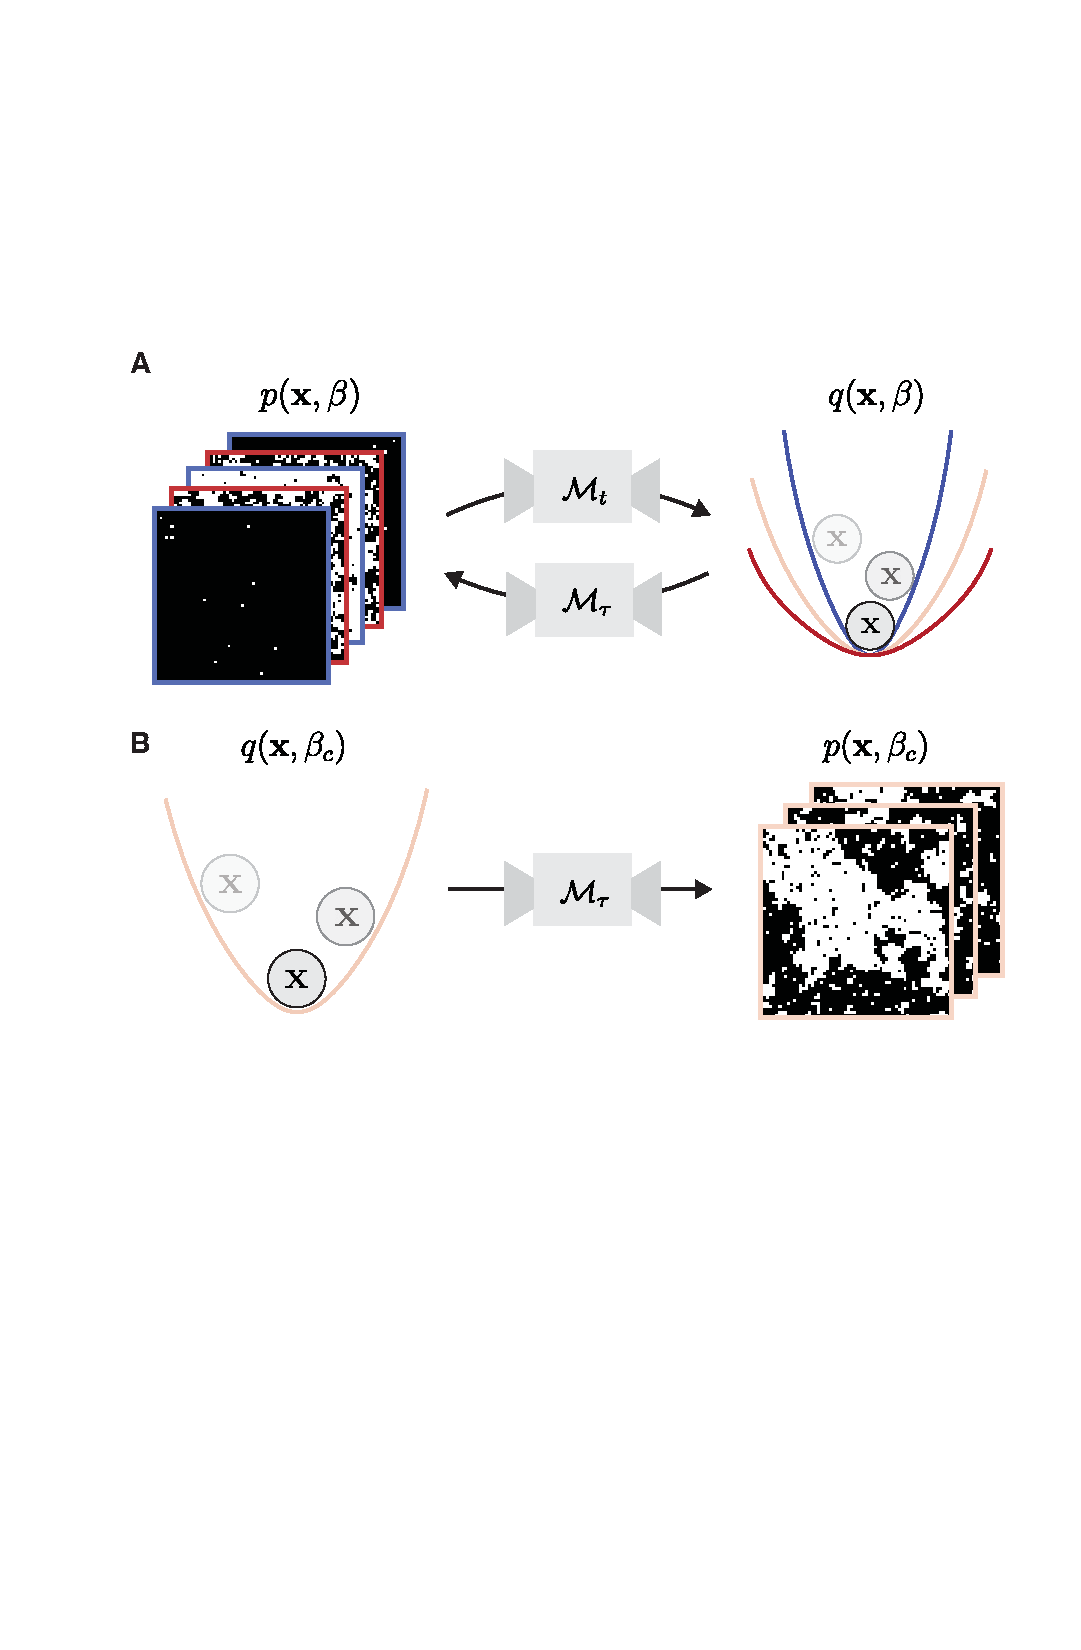
\includegraphics[
    width=0.74\textwidth
    ]{figures/ch4_ising-figure.pdf}
    \caption{{\bf Illustration of a thermodynamic map between systems.} {\bf A} The thermodynamic map is parameterized as a score-based model transporting densities from a target distribution  $p(\mathbf{x}, \beta)$ to a prior distribution $q(\mathbf{x}, \beta)$.  In the schematic, data from an Ising model at two temperatures is mapped onto a simple harmonic oscillator. The generative process $\mathcal{M}_\tau$ is parameterized from realizations of the forward process $\mathcal{M}_t$. {\bf B} Once learned, the thermodynamic map allows samples of the complex system to be generated from the simple prior system at any temperature -- even those showing non-trivial behavior -- by sampling the prior at the correct temperature.}
    \label{ch4:fig:schematic}%
\end{figure*}

\label{ch4:sec:TM}

The Einstein-Smoluchowski relation states that temperature is proportional to the diffusivity of a Brownian motion \cite{dill2010molecular}. Accordingly, we introduce temperature to the SBM SDEs (Eqs. \ref{ch4:eq:FPE-SDE} and \ref{ch4:eq:FPE-SDE-bck}) by augmenting the positions $\mathbf{x}\in \mathbb{R}^{d}$ with auxiliary inverse temperature-type variables $\bm{\beta}\in \mathbb{R}^{d}$. Together, the coordinates and temperatures form a state vector $(\mathbf{x},\bm{\beta})^\top \in \mathbb{R}^{2d}$, and the thermodynamic map is parameterized in the joint $\mathbf{x}$-$\bm{\beta}$-space as a SBM of the form

\begin{align}
\label{ch4:eq:sde-fwd}
\begin{pmatrix}
    \text{d}\mathbf{x}\\
    \text{d}\bm{\beta}^{-1}
\end{pmatrix}
 &= -\lambda(t)
\begin{pmatrix}
    \mathbf{x}\\
    \bm{\beta}^{-1}
\end{pmatrix}
\text{d}t \nonumber \\\quad &+ \sqrt{2\lambda(t)}
\begin{pmatrix}
    \sqrt{\bm{\beta}_0^{-1}}\\
    \mathbf{1}
\end{pmatrix}\text{d}\mathbf{B}_t\quad \text{and}
\end{align}

\begin{align}
\label{ch4:eq:sde-bck}
\begin{pmatrix}
    \text{d}\mathbf{x} \\
    \text{d}\bm{\beta}^{-1}
\end{pmatrix}
&= - \lambda(\tau) \left[
    \begin{pmatrix}
        \mathbf{x} \\
        \bm{\beta}^{-1}
    \end{pmatrix}
    + \mathbf{s}_{\theta}(\mathbf{x}, \bm{\beta}^{-1}, \tau)
\right] \, \text{d}\tau \nonumber \\
&\quad + \sqrt{2\lambda(\tau)}
    \begin{pmatrix}
        \sqrt{\bm{\beta}_0^{-1}} \\
        \mathbf{1}
    \end{pmatrix}
    \, \text{d}\mathbf{B}_\tau.
\end{align}

Both $\mathrm{x}$ and $\bm{\beta}$ fluctuate during the dynamics of Eqs. \ref{ch4:eq:sde-fwd} and \ref{ch4:eq:sde-bck}, relaxing to $\mathcal{N}(\mathbf{0}, \bm{\beta}_0^{-1})$ and $\mathcal{N}(\mathbf{0}, \mathbf{1})$ respectively at $t=1$. The value of the auxiliary variables $\bm{\beta}$ at $t=0$ is denoted by $\bm{\beta}_0$ and is a constant that sets the temperature of the diffusive dynamics for each component of $\mathbf{x}$ by rescaling the Brownian motion. The construction ensures that the diffusion process for $\mathbf{x}$ relaxes to a normal distribution at temperature $\bm{\beta}_0^{-1}$.
}

% The auxiliary variables scale the Brownian motion, ensuring that starting from initial conditions $\mathbf{x}_0$ and $\bm{\beta}_0$ at $t=0$, the distributions for the coordinate and temperature variables relax to $\mathcal{N}(\mathbf{0}, \bm{\beta}_0^{-1})$ and $\mathcal{N}(\mathbf{0}, \bm{1})$ at $t=1$.
% {\pt does this mean that beta has mean 0 or temperature is approaching infinite? clarify }
 
%With Eq. \ref{ch4:eq:sde-fwd}, it is trivially easy to corrupt data samples to noise, and Eq. \ref{ch4:eq:sde-bck} allows for the diffusion to be reversed and for noise samples to be transformed into data samples. However, the gradients of the probability distribution for each $t$ are required to evaluate Eq. \ref{ch4:eq:sde-bck}. Since the data distribution has no closed form expression, $\nabla_{\mathbf{x}}\log p_t(\mathbf{x})$ and $\nabla_{\bm{\beta}}\log p_t(\bm{\beta})$, commonly referred to as ``scores'', must be estimated for each $t$. Score-based models (including diffusion models) estimate these gradients using deep neural networks.

A thermodynamic map maps the thermodynamics of a target system $p(\mathbf{x},\bm{\beta})$ onto the thermodynamics of a simple prior system $q(\mathbf{x}',\bm{\beta}')$, where in both systems each degree of freedom is coupled to separate baths defined by $\bm{\beta}$. Our construction is motivated by treating the prior distribution as the equilibrium distribution arising from the dynamics of a physical system. If the prior is a Gaussian distribution then the corresponding physical system is a simple harmonic oscillator, and generating samples from $p(\mathbf{x})$ at $\bm{\beta}$ amounts to sampling from the harmonic oscillator $q(\mathbf{x}')$ at the corresponding $\bm{\beta}'$. Details on training and inference are provided in SI Appendix A.

In the generalized construction above we have assumed that each degree of freedom of $\mathbf{x}$ is coupled to a separate bath defined by the entries of $\bm{\beta}$, but in most cases physical systems are coupled to a single bath. If samples of $p(\mathbf{x},\bm{\beta})$ are from the global equilibrium distribution of an ensemble defined by $\beta_\mathrm{bath}$, each entry of $\bm{\beta}$ should be equal to $\beta_\mathrm{bath}$. However, global equilibrium distribution is often not attainable in practice (e.g. in molecular dynamics simulations). In this case, allowing each degree of freedom of $\mathbf{x}$ to be coupled to separate baths $\bm{\beta}$ allows the global equilibrium distribution to be inferred from samples gathered under a local equilibrium distribution. In SI Appendix G we discuss how the global equilibrium distribution can be inferred from local equilibrium samples if one assumes that $\bm{\beta}$ varies linearly with $\beta_{\mathrm{bath}}$. In Section \ref{ch4:sec:RNA} we demonstrate the validity of the assumption by inferring the global equilibrium distribution from short, independent molecular dynamics simulations of two RNAs.

\subsection{Critical Behavior of the Ising Model}
\label{ch4:sec:ising}

We apply thermodynamic maps to the most widely studied formulation of the classical Ising model as a system of interacting spins arranged on a two-dimensional square lattice, without the presence of an external magnetic field. Arguably, this model serves as a prototypical example of a simple system with a complex phase transition. Each spin can have one of two states with value $\sigma=+1$ or $\sigma=-1$, and the spins interact with their nearest neighbors through an interaction term $J$ and Hamiltonian given by 
\begin{equation}
    \mathcal{H} = J\sum_{\langle i,j\rangle } \sigma_i \sigma_j,
\end{equation}
where $\langle i,j\rangle$ denotes nearest-neighbor pairs. When $J<0$ the model exhibits ferromagnetic behavior in its ground state. Going forward, we set $J=-1$ without loss of generality.
\begin{figure*}
    \centering
    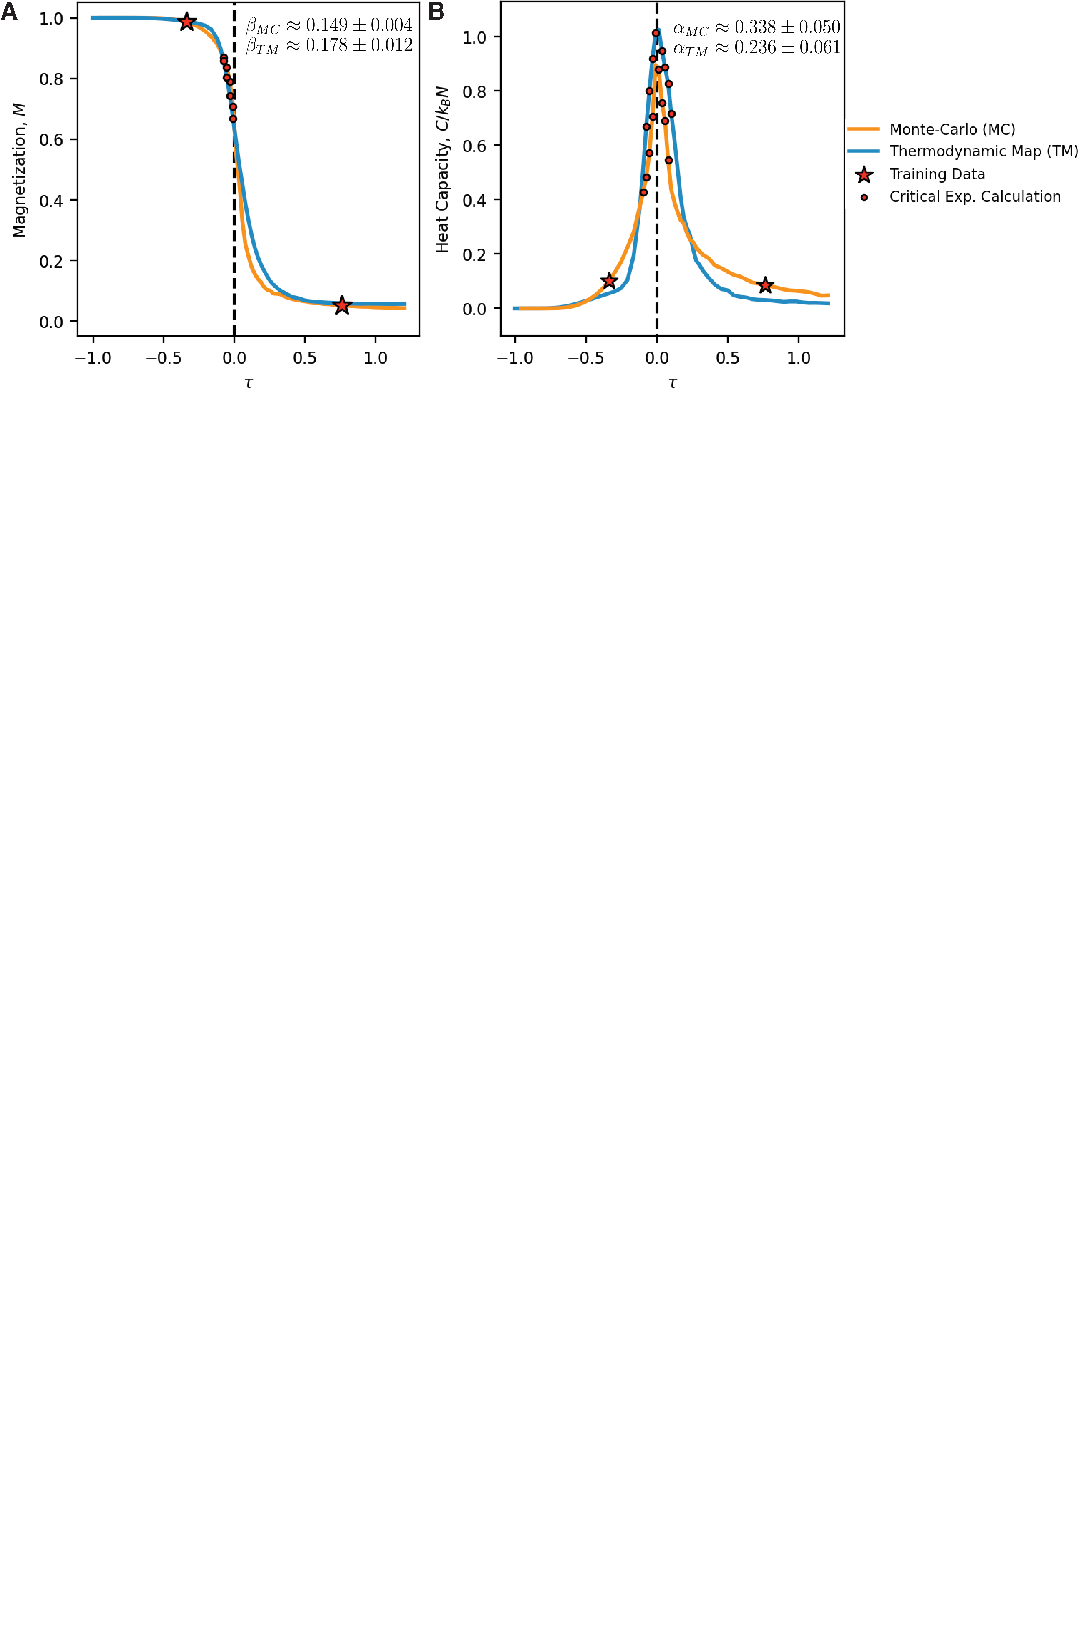
\includegraphics[
    width=\textwidth
    ]{figures/ch4_Figure-mag-and-heat-cap.pdf}
    \caption{{\bf Inferring the phase transition of the 2D Ising model from limited sampling.} {\bf A} The magnetization is plotted for samples of a $32\times32$ square Ising model generated through MC sampling (orange) and the thermodynamic map (blue). The thermodynamic map predicts change in magnetization at $T_c$ when trained on samples generated at $T=1.5$ and $T=4$ (red stars). Similar results were obtained (not reported) for a symmetric choice of training data temperatures. {\bf B} The heat capacity of samples generated from MC sampling (orange) and the thermodynamic map (blue) is plotted. The thermodynamic map infers the divergence in the heat capacity, numerically computed for the red dots, when trained on the same samples as panel A (red stars).}
    \label{ch4:fig:ising-model-mag}%
\end{figure*}

As the temperature increases, an Ising model in two or higher dimensions transitions from an ordered magnetic phase to a disordered paramagnetic phase. For our set-up of a two-dimensional Ising model on a square lattice with $J=-1$, this critical temperature is known to be $T_c\approx2.27$ \cite{onsager-solution}. The two phases can be distinguished from each other with the magnetization order parameter, $M$, defined as the absolute value of the average of the spins. Well above $T_c$, as $T \rightarrow \infty$, the spins are equally likely to be $+1$ or $-1$, regardless of their neighbors, resulting in a net magnetization of zero. Well below $T_c$, all spins in the lattice align, leading to a magnetization of 1. Power law scaling is a signature of critical behavior, and near the critical temperature the magnetization $M$ and heat capacity $C$ of the Ising model scale as:
\begin{equation}
    M \sim |\tau|^{\beta} \quad \mathrm{and} \quad C \sim |\tau|^{-\alpha} \quad \mathrm{where} \quad \tau = \frac{T-T_c}{T_c},
\end{equation}
and with critical exponents $\alpha=0$ and $\beta=0.125$ {(not to be confused with the inverse temperature variables $\bm{\beta}$), which can be derived analytically in the thermodynamic limit \cite{ising-crit-exp}. For systems that are not solvable, the critical exponents must be measured numerically, which is often done through MC sampling, wherein proposals for spin flips are generated and their acceptance or rejection is determined based on the detailed balance condition. Near the critical temperature, the presence of long-range correlations causes MC dynamics to slow down exponentially, leading to difficulty in sampling the phase transition \cite{wolff-critical-slow-down}.

We investigate the ability of thermodynamic maps to infer such critical behaviors by generating configurations of an Ising model through MC sampling across temperatures and using the data from two temperatures asymmetrically spaced about $T_c$ to train a TM (details provided in SI Appendix C). In the formalism of Eqs. \ref{ch4:eq:sde-fwd} and \ref{ch4:eq:sde-bck} the lattice configurations are $\mathbf{x}_0 \in \mathbb{R}^{32\times32}$ and each entry of $\bm{\beta}_0^{-1} \in \mathbb{R}^{32\times32}$ is the bath temperature; a straightforward choice since MC sampling guarantees the global equilibrium distribution. Once the TM is trained, we generate configurations at each temperature by evaluating Eq. \ref{ch4:eq:sde-bck} with each entry of $\bm{\beta}_0^{-1}$ equal to $T_{\mathrm{bath}}$. The generated continuous-valued configurations $\mathbf{x}$ are then transformed into discrete spins by $\sigma = \mathrm{sgn}(\mathbf{x})$, and the average magnetization and heat capacity at each temperature is estimated directly from the spin configurations. Figure \ref{ch4:fig:ising-model-mag} shows the behavior of $M$ and $C$ for the MC and TM-generated samples. The TM infers the correct value of $T_c$ ($\tau=0$) even based on limited, deliberately misleading training data and generates samples with divergences in $M$ and $C$. 

Figure \ref{ch4:fig:ising-model-mag}A shows the behavior of the magnetization for MC and TM-generated samples across temperatures, with critical exponents measured as $\beta_{MC} \approx 0.149 \pm 0.004$ and $\beta_{TM} \approx 0.178 \pm 0.012$. Similarly, Figure \ref{ch4:fig:ising-model-mag}B shows a divergence in the heat capacity at $T_{MC}\approx2.25$ and $T_{TM}\approx2.30$, with critical exponents $\alpha_{MC} \approx 0.338 \pm 0.050$ and $\alpha_{TM} \approx 0.236 \pm 0.061$. For both exponents, the MC and TM exponents agree with each other, although far from the ideal value due to finite size effects.

These results highlight the ability of our model to infer the non-trivial thermodynamic behavior of phase transitions without being shown samples from the transition region; the physical meaning of temperature in the prior system has been transferred to the complex system, complete with the statistics properties associated with critical behavior. The correct prediction of $T_m$, even with asymmetrically spaced training temperatures, indicates our model has learned the physics of the Ising model, not merely the distribution of structures at each temperature.

\subsection{Exploring RNA Conformational Landscapes with Thermodynamic Map-accelerated Molecular Dynamics (TM-aMD)}
\label{ch4:sec:RNA}

\begin{figure*}[h!]
    \centering
    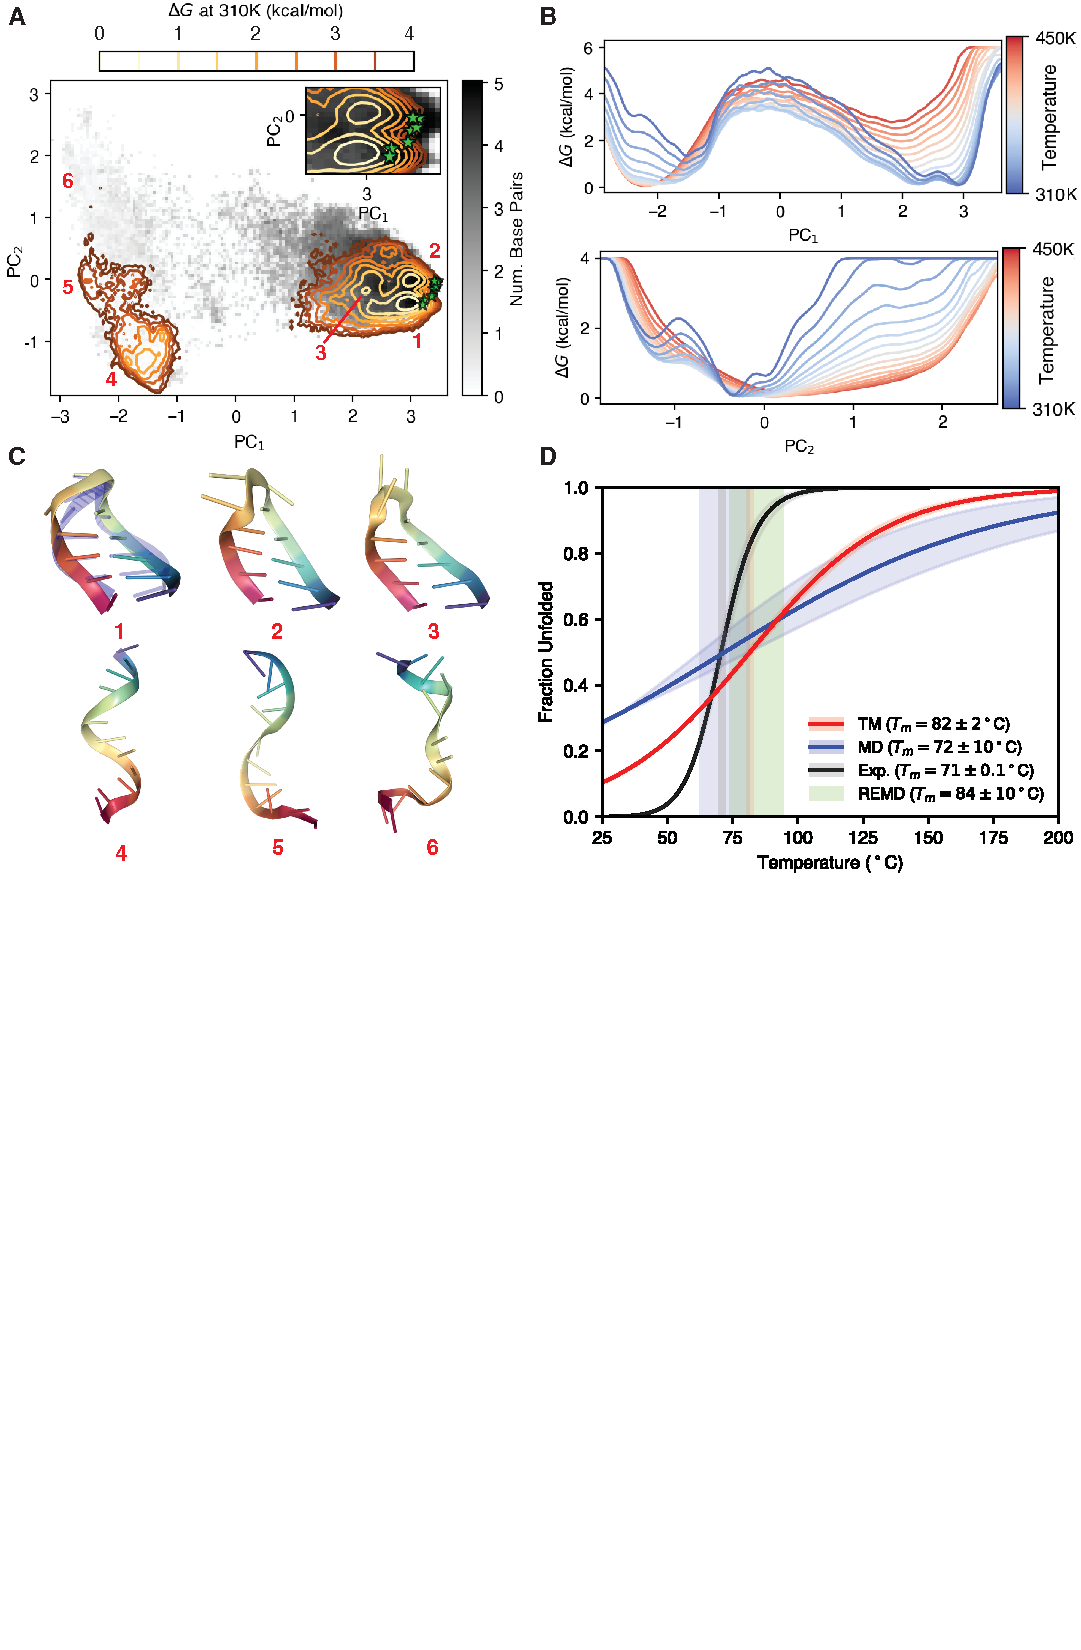
\includegraphics[
    width=\textwidth
    ]{figures/ch4_Figure-GCAA-final.pdf}
    \caption{{\bf GCAA Tetraloop Conformational Landscape.} {\bf A} Joint distribution of the first two principal components of G-vectors for GCAA. Contours representing TM-generated samples at 310K are overlaid on MD samples shaded by the number of base pairs, with selected regions of the conformational landscape annotated as 1-6. The 10 NMR conformers reported in the Protein Data Bank (PDB: 1ZIH) are depicted as green stars. {\bf B} Temperature-dependent free energy profiles along the first two principal components shown in panel A. Colors indicate temperatures ranging from 310K to 450K at 10K intervals. {\bf C} Representative structures sampled from labeled minima in panel A, with a representative NMR conformer shown in translucent blue. The structures are colored from blue to red from the 5' to 3' end. {\bf D} A fraction unfolded curve is obtained by reweighting the MD data in panel A with the TM conformational ensemble for each temperature in panel B, and fitting a two-state model. Uncertainties are computed from the last three iterations of TM-aMD. The cutoff for folded and unfolded states is three base pairs to match a reference REMD study \cite{DE-Shaw-RNA-ff}.}
    \label{ch4:fig:gcaa}%
\end{figure*}

To show the broad applicability of thermodynamic maps, we now study conformational transitions and melting in two different ribonucleic acid (RNA) systems. Studying atomic-resolution conformational ensembles of RNAs through molecular dynamics simulations has proved crucial for understanding RNA structural dynamics, yet remains challenging due to the disordered, glassy nature of RNA energy landscapes \cite{DE-Shaw-RNA-ff,bussi-ff-deficiency}.
% Reaching longer timescales in RNA simulations has proved essential for understanding the complexity of RNA structural dynamics.

Increasing evidence points towards some RNAs having glassy energy landscapes where multiple minima are separated by high barriers \cite{kremer-polymer,parisi-RNA,wales-RNA}. The ruggedness of the landscape results in many competing degrees of freedom and no clear-cut separation of timescales within the dynamics \cite{hashimi-glass,wales-RNA,parisi-RNA}. The most striking feature of glassy energy landscapes as they relate to polymers is the presence of conformational heterogeneity at equilibrium \cite{parisi-RNA, kremer-ML};  while the conformational landscape of proteins is often dominated by a single well-defined fold (energy minimum), the RNA conformational landscape may not be dominated by a single structure \cite{hashimi-invisible,hashimi-nmr-dock}. This difference is analogous to the single magnetized phase of an Ising model and the multiple phases of long-ranged spin glasses \cite{parisi-replica-trick, ANNNI,hopfield-network,amit-spin-glass}.  Since multiple members of the ensemble contribute substantially to the free energy and other thermodynamic observables, RNAs are best described as a weighted ensemble of conformers \cite{how-to-think,hashimi-nmr-dock}. 

Exploring energy landscapes by biasing dynamics along a small number of slow degrees of freedom has proven successful for exploring the conformational landscape of proteins, but the lack of timescale separation and ensemble nature of the RNA conformational landscape violates fundamental assumptions of dimensionality made in biasing methods \cite{metadynamics-review}. On the other hand, thermodynamic maps have the advantage of being able to learn the conformational landscape directly in a much higher-dimensional configuration space.

We train thermodynamics maps on limited information generated by bioinformatic approaches and multi-ensemble molecular dynamics simulations to efficiently characterize RNA conformational ensembles. Our starting point is the physics and knowledge-based potential that is central to Rosetta to generate a putative conformational ensemble \cite{rosetta}. These structures serve as the starting point to explore a more realistic energy landscape through all-atom, explicit solvent molecular dynamics performed over a range of temperatures. Between rounds of molecular dynamics simulation, the global equilibrium distribution is inferred using thermodynamic maps alongside assumptions of local equilibrium (see SI Appendix G). Initial conditions are re-sampled from the inferred equilibrium distribution using a geometric RNA order parameter. Here on, we refer to this protocol as thermodynamic map-accelerated Molecular Dynamics (TM-aMD).

Although agreement between the input equilibrium distribution and the output from the thermodynamic map is a necessary, though not sufficient condition that the true equilibrium distribution has been attained, we leave rigorously addressing convergence to equilibrium to future work. Here we take solace in the numerical results for the two challenging test systems, described next. 

\subsubsection{GCAA Tetraloop}

With a shift in perspective towards viewing RNAs as dynamic entities, there has been interest in studying the variation in dynamics between different tetraloops. Studies combining computation and experiment have demonstrated that even so-called simple tetraloops can exhibit rich dynamics \cite{kresten-jacs}. We study the GCAA tetraloop, a well-studied model system, enabling us to compare the equilibrium distribution generated by our model with extensive molecular dynamics simulations and experimental data \cite{debenedetti-rna,DE-Shaw-RNA-ff,gcaa-melt}. The GCAA Tetraloop is a small, highly-stable, 12-nucleotide RNA sequence that adopts a hairpin structure consisting of an eight-nucleotide helix and a four-nucleotide loop (PDB: 1ZIH) \cite{gcaa-nmr}. Consistent with an ensemble perspective, the variable arrangement of nucleotides in the loop gives rise to alternative conformations, which we investigate with TM-aMD.

The thermodynamic map learns to generate RNA structures represented as $G$-vectors -- an internal coordinate system for RNAs that effectively clusters distinct folded states \cite{gvecs-bussi}. The principal components of $G$-vectors have been shown to be a convenient visualization of RNA structural diversity, which we use to guide adaptive sampling. Further information on $G$-vectors, along with details of TM-aMD can be found in the SI Appendix D.

Figure \ref{ch4:fig:gcaa} summarizes the result of nine iterations of our enhanced sampling procedure, with a total of 50$\mu$s of simulation. Although we performed extensive MD simulations reaching long timescales, we still used two orders of magnitude less compute compared to our reference millisecond replica exchange simulation, even with sub-optimal scheduling of TM learning with MD simulation  \cite{DE-Shaw-RNA-ff}. Figure S2A suggests that TM-aMD would benefit from more frequent reseeding of simulations.

In Figure \ref{ch4:fig:gcaa}A, we present the projection of the learned equilibrium distribution onto the first two principal components of the $G$-vectors. The contours represent the free energy landscape inferred by the thermodynamic map, while the shaded regions represent the distribution of structures observed in the simulation, shaded by the number of base pairs. The 10 conformers reported in the Protein Data Bank (PDB), represented as green stars, lie within the most dominant TM-predicted cluster. Figure \ref{ch4:fig:gcaa}B shows the learned, temperature-dependent free energy profiles along each of the principal components in Figure \ref{ch4:fig:gcaa}A. The first principal component clearly shows the reweighting of the folded and unfolded states with temperature. Figure \ref{ch4:fig:gcaa}C shows the structures associated with the minima in Figure \ref{ch4:fig:gcaa}A. The first three conformations are abundant at 310K and are consistent with MD studies \cite{DE-Shaw-RNA-ff,debenedetti-rna} and experiment (an example NMR conformer is depicted in blue). The last three represent unfolded states that are stabilized by base stacking and are weakly present in the 310K ensemble. The first principal component corresponds to the folding-unfolding transition, while the second captures the conformational heterogeneity of the loop region.

Figure \ref{ch4:fig:gcaa}D displays the melting curve of the GCAA tetraloop computed from the last three rounds of MD simulation, with the melting curve of the learned equilibrium distribution. Both curves exhibit agreement, matching the range of melting temperatures predicted from a millisecond Replica Exchange Molecular Dynamics (REMD) simulation conducted with the same force-field \cite{DE-Shaw-RNA-ff}. However, both the TM-generated melting curve and the range of melting temperatures from the reference are higher than the experimental melting temperature, indicating that current force-fields do not yet accurately capture the temperature dependence of the tetraloop ensemble.
%Our estimation of the melting temperature has lower uncertainty compared to the replica exchange study and requires only a fraction of the computational resources {\pt quantify clearly esp in light of the 50 microsec comment above}.

% {\pt done till here in this round. by aug 10, please finish remaining parts after here and make all changes above. then i will start again from beginning}
\subsubsection{HIV-TAR RNA}

\begin{figure*}[h!]
    \centering
    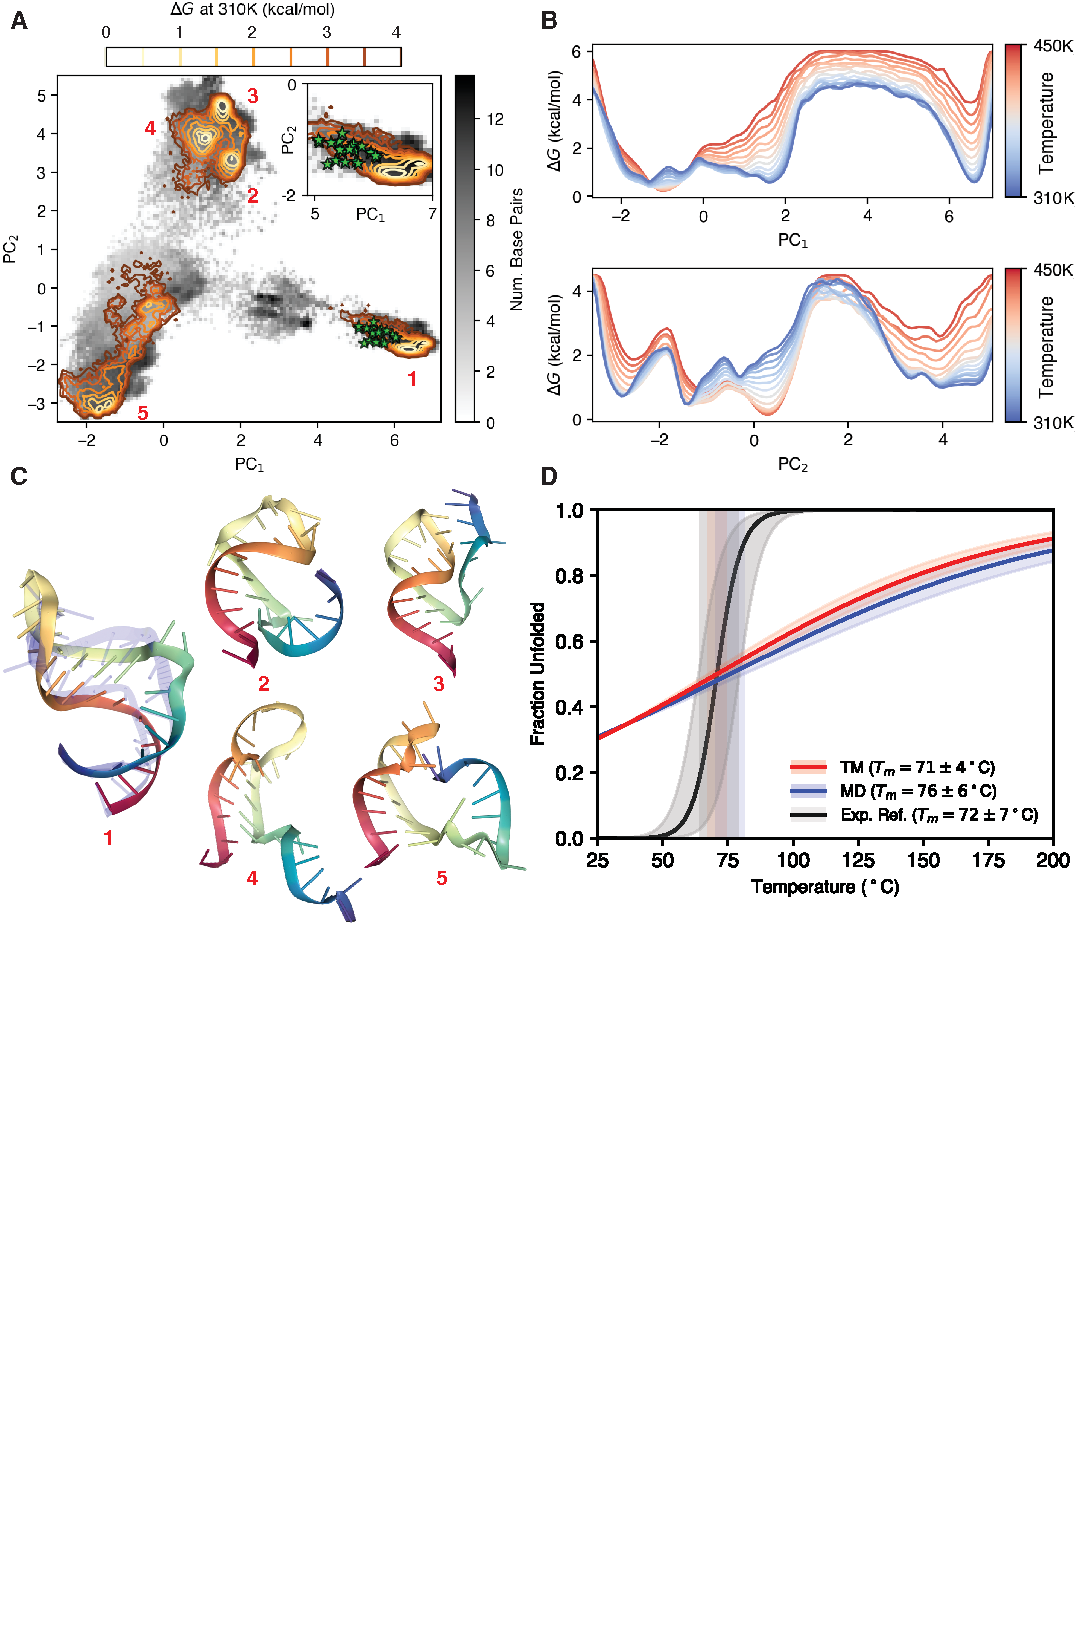
\includegraphics[
    width=\textwidth
    ]{figures/ch4_Figure-hiv-tar-final.pdf}
    \caption{{\bf HIV-TAR RNA Conformational Landscape.} {\bf A} Joint distribution of the first two principal components of G-vectors for HIV-TAR. Contours representing TM-generated samples at 310K are overlaid on MD samples shaded by the number of base pairs, with basins of the TM landscape labeled 1-5. The 20 reported NMR conformers in the Protein Data Bank (PDB: 1ANR) are depicted as green stars. {\bf B} Temperature-dependent free energy profiles along the first two principal components are shown in panel A. Colors indicate temperatures ranging from 310K to 450K at 10K intervals. {\bf C} Representative structures sampled from labeled clusters in panel A, with a representative NMR conformer shown in translucent blue. The structures are colored from blue at the 5' end to red at the 3' end.  {\bf D} A fraction unfolded curve is obtained by reweighting the MD data in panel A with the TM conformational ensemble for each temperature in panel B, and fitting a two-state model. Uncertainties are computed from successive iterations of the TM-aMD algorithm showing agreement between MD and TM-predicted melting temperatures (see Figure S2B). The cutoff for folded and unfolded states is nine base pairs, as determined by the NMR conformers).}
    \label{ch4:fig:hiv}%
\end{figure*}

The HIV-TAR RNA is an extensively studied, 29 nucleotide RNA hairpin from the HIV genome that displays rich conformational diversity. The secondary structure consists of lower and upper helices separated by a three-nucleotide bulge with an apical loop closing the upper helix (PDB: 1ANR) \cite{hiv-nmr}. The disordered loop and bulge regions mediate interactions with proteins and small molecules \cite{hiv-tar-binding}. We investigate the conformational landscape of the HIV-TAR RNA using six iterations of TM-aMD, requiring a total of 70$\mu$s of simulation time. We infer relative free energies between the dominant conformer observed through NMR spectroscopy and alternative conformers, which are unattainable through MD simulation alone.

The conformational landscape predicted by the learned TMs, projected along the principal components of the $G$-vectors is shown in Figure \ref{ch4:fig:hiv}A. Structures corresponding to the NMR ensemble (green stars) are well-separated from other misfolded structures within the two-dimensional projection. The temperature dependence of the free energy along each principal component is shown in Figure \ref{ch4:fig:hiv}B, where we find that the free energy barrier separating the NMR conformers from unfolded states reaches a height of $5$kcal/mol. Figure \ref{ch4:fig:hiv}C depicts representative samples from each cluster.  The first cluster shows agreement with the NMR conformers, with the first reported conformer shown in translucent blue. The other clusters correspond to varied secondary structure motifs. Generally, across the conformational landscape, we find that the contribution of folded states to the conformational ensemble diminishes as temperature increases. This can be clearly shown by computing a fraction folded curve (Figure \ref{ch4:fig:hiv}D), which shows agreement between melting temperatures of the MD and TM-derived ensembles, and the experimental melting temperature \cite{hiv-experiment}.

Our results support the idea that RNAs evolve over a rugged free energy landscape punctuated by many long-lived states \cite{dill-chen}. We find that the native state is indeed the most stable at physiological temperatures ($310$K), but misfolded states consisting of secondary structure elements still have substantial contributions to the ensemble. Minima of the energy landscape corresponding to states 2-5 in Figure \ref{ch4:fig:hiv} differ from the NMR conformers (state 1) by less than $1$kcal/mol. Overall, our findings are in agreement with theoretical studies of RNA folding pointing towards a rugged energy landscape \cite{dill-chen,wales-RNA}.

Clearly, our findings are dependent on the accuracy of the simulation force field, which for RNAs have not yet reached experimental accuracy. Moreover, TM-aMD is incapable of reaching experimental folding timescales. Despite this, the fraction folded curve for HIV-TAR agrees with experimental results \cite{hiv-experiment}. Improved forcefields are out of reach due to the difficulty of attaining equilibrium through simulation; a potential application for TM-aMD may be accelerating convergence to equilibrium, allowing for more rapid evaluation of force-field parameters.

\section{Discussion}

We have demonstrated that thermodynamic maps (TMs) are capable of inferring the non-trivial behavior of the free energy with temperature from limited data for the two-dimensional square Ising model. Additionally, we also show how thermodynamic maps may be integrated with molecular dynamics simulation to enhance sampling. In this section, we outline prospective, potential applications for thermodynamic maps. Our experiments for inferring critical behavior in the Ising model suggest a number of potential research directions that might shed light on some general principles underpinning thermodynamic maps. We outline three directions below.

In this work, we have not explored the mechanism by which thermodynamic maps learn phase transitions. In Section \ref{ch4:sec:ising}, as the Ising lattice grows larger the ability to infer the phase transition from only two observations diminishes. Inversely, as the lattice size decreases, the phase transition is learned more consistently. These observations suggest a connection between fluctuations due to finite-size effects and robustness of the algorithm. Spin-glasses with multiple phases present a setting for exploring these connections without the additional complexity molecular dynamics brings.

A second avenue worth exploring the extent to which thermodynamic maps infer dramatic changes in Boltzmann weights across temperature. Here too, spin-glasses are an appealing system; some spin-glasses exhibit temperature chaos, where, in the thermodynamic limit, the weights change discontinuously with temperature \cite{ritort-temperature-chaos}. In the framework provided in the introduction, this behavior manifests as a phase transition (i.e. a discontinuity in $Z(\beta)$). Recently, descriptions of temperature chaos have been generalized to finite systems, where it is prevalent on a characteristic length scale that diverges as the change in temperature becomes infinitesimal \cite{parisi-temperature-chaos}.

Another direction closely related to those outlined above is determining if thermodynamic maps can capture critical behavior arising from correlation functions. The order parameters explored in this work (magnetization and heat capacity) are measured by averaging over the entire system, but critical exponents are derived from the asymptotic behavior of correlation functions that capture the microscopic details of fluctuations. To measure some critical exponents, computing correlation functions is unavoidable.

In terms of applications, our results in Section \ref{ch4:sec:RNA} obtained by TM-aMD indicate that thermodynamic maps are well suited for inferring equilibrium distributions from swarms of short, independent simulations. We show that TM-aMD is capable of exploring the conformational landscape orders of magnitude faster than REMD, and inferring global equilibrium from samples gathered under local equilibrium. Still, TM-accelerated MD stands to benefit greatly from optimization. And since TMs allow for truly parallel simulations across arbitrary temperatures, TMs are poised to make efficient use of distributed computing resources \cite{folding-at-home}. 

As pointed out in Section \ref{ch4:sec:RNA}, we believe that our implementation of TM-aMD is hindered by the scheme used to adaptively re-sample initial states. The one we employ aims for agreement between the TM and MD-generated distributions. However, in practice it is more productive to balance thermodynamic accuracy with sampling of diverse conformations. Methods such as FAST and REAP quantify this trade-off as a reward function which is to be optimized by the choice of adaptive sampling strategy \cite{FAST,REAP}.

Finally, as presented, thermodynamic maps are not informative of kinetics since the samples they generate are independent. In principle, one may use the height of the barrier separating states and recrossing related dynamical corrections to estimate rates \cite{berne1988classical}. Still, we do not expect this approach to be useful without some form of further enhanced sampling \cite{tiwary2013metadynamics}.

Overall, we have presented thermodynamic maps as an exciting way of integrating score-based generative modeling with the theoretical framework of statistical mechanics. We have demonstrated the capability of thermodynamic maps to learn physics by predicting the critical behavior associated with the Ising Model despite limited, deliberately misleading sampling. We also use thermodynamic maps to accelerate Molecular Dynamics (TM-aMD) and show that TM-aMD efficiently infers the equilibrium distribution of two model RNA systems using a fraction of the computational resources required by replica exchange simulations. The TM-aMD method, combined with experimentally measured melting curves, might also prove useful for improving force fields for RNA and similar systems. Based on these results, we believe that thermodynamic maps are suitable for widespread use and have great potential for further theoretical development and computational optimization.

{https://github.com/tiwarylab/thermomaps-ising}.}

% \section{Code Availability}
% A Python implementation of a thermodynamic map trained to predict the phase transition of the Ising model is made available for public use at \href{https://github.com/tiwarylab/thermomaps-ising}{https://github.com/tiwarylab/thermomaps-ising}.

 % Display the acknowledgments section

% \bibsplit[2]
%Use \bibsplit to split the references from the body of the text. Value "[2]" represents the number of reference in the left column (Note: Please avoid single column figures & tables on this page.)

% Bibliography